\begin{document}
\renewcommand{\dept}{icis}

\bibliographystyle{plain}

% Load literature in temporary savebox to prevent generation of new frame
\newsavebox\mytempbib
\savebox\mytempbib{\parbox{\textwidth}{\nobibliography{literature}}}
\pagecolor{white}
\begin{frame}
    \titlepage
    
    \pnote{
        Welcome to my thesis presentation.\\
        Today I'll present my work on developing a system for premise selection for the ITP Coq.
    }
\end{frame}

\begin{frame}{Outline}
	\begin{itemize}
		\item What is Premise Selection?
		\item How to do Premise Selection for Coq?
		\item Contributions
		\item Results
    \end{itemize}
    
    \pnote{
        First I'll explain what this thesis is about.\\
        Then how it is done for the ITP Coq, known by our bachelor students.\\
        I'll quickly summarize the contributions made in this thesis.
        And finally I'll finish with an overview of the achieved results.\\
        This will take approximately 30 minutes, and then I'll open up the floor for questions.\\
    }
\end{frame}

\begin{frame}{Proofs}
	\begin{minipage}{0.5\textwidth}
		\begin{itemize}
			\item All men are mortal.
			\item Socrates is a man.
			\item Therefore, Socrates is mortal.
		\end{itemize}
	\end{minipage}
	\hspace{2em}
	\begin{minipage}{0.4\textwidth}
		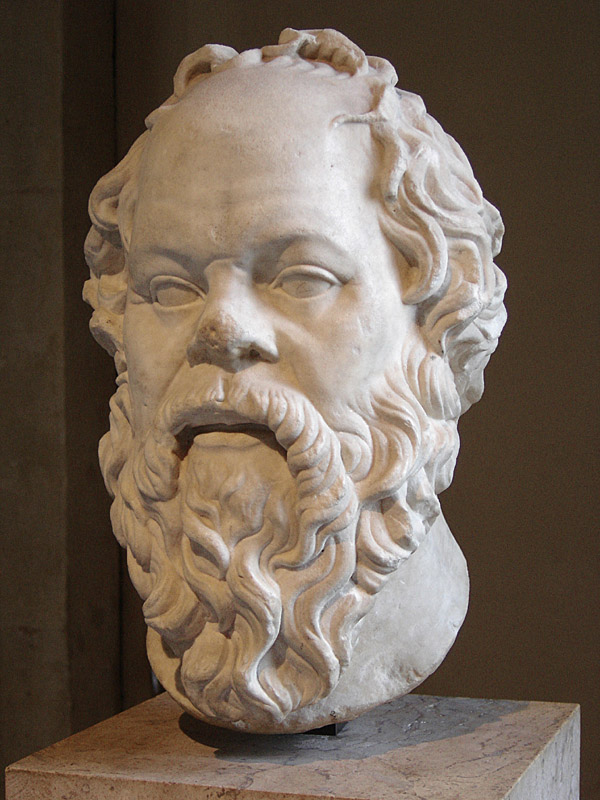
\includegraphics[width=1.0\textwidth]{figures/socrates.jpg}\\
		\centering \color{gray}{Eric Gaba (CC by-nc-sa 2.5)}
    \end{minipage}

    \pnote{
        First off, let's look at some fundamentals.\\
        Some mathematicians concern themselves with proofs.\\
        A proof is an argument for a mathematical statement to be true.\\
        In this example, Socrates is mortal is a premise, that follows logically from the two base truths.\\
        These base truths are called axioms.\\
        A premise is assumed to be true, but need not be proven (yet).\\
        Truths based on other truths are called theorems, thus when proven, this premise will become a theorem.\\
        In this case, the argument itself is considered to be an informal proof, as it is dependant upon informal language.\\
        Actually the entire argument is contained in the word 'therefore', which is an implication that the latter follows from the former.\\
        Informal proofs are sometimes error prone, and mathematicians try to vigorously check such informal proofs.
    }
\end{frame}

\begin{frame}{Propositional logic}
	\begin{block}{Primitives}
			Atomic values: $P, Q$\\
			Operations: $\rightarrow$\\
			Term: $P \rightarrow Q$\\
			Derivation: $H_1, \dots, H_n \vdash P$
    \end{block}
    
    \pnote{
        Alternatively, mathematicians have developed systems for formal proofs.\\
        In this case, we have a simple logic, propositional logic.\\
        \\
        There are values, say 'Socrates' and 'man'.\\
        Operations, such as the implication.\\
        A term is either a value, or composed out of other terms and operations.\\
        And from that we can derive truths, in this case, P follows from several hypothesis.
    }

	\uncover<2->{
	\begin{block}{Proof rules}
			\begin{center}
					\begin{minipage}{.4\textwidth}
					\[
							\begin{prooftree}
									\justifies
									H, P \vdash P
									\using \text{hyp}
							\end{prooftree}
					\]
					\end{minipage}
					\begin{minipage}{.4\textwidth}
							\[
									\begin{prooftree}
											H, P \vdash Q
											\justifies
											H \vdash P \rightarrow Q
											\using \rightarrow \text{intro}
									\end{prooftree}
							\]
					\end{minipage}\\
					\vspace{1em}
					\begin{minipage}{1.0\textwidth}
					\[
							\begin{prooftree}
											H, \vdash P \rightarrow Q
											\hspace{1em}
											H \vdash P
											\justifies
											H \vdash Q
											\using \rightarrow \text{elim}_{[P]}
							\end{prooftree}
					\]
					\end{minipage}
			\end{center}
    \end{block}
    
    \pnote{
		------------\\
        And to prove this, we have several derivation rules.\\
        We can apply these rules to form a proof.\\
        Something is proven if these rules are correctly applied, and all subderivations are closed.
    }
	}
\end{frame}

\begin{frame}[fragile]{Propositional logic \small{example}}
	\begin{block}{Theorem}
			\[ (P \rightarrow Q) \rightarrow P \rightarrow Q \]
	\end{block}
	\begin{block}{Proof}
			\[
					\begin{prooftree}
							\begin{prooftree}
									\begin{prooftree}
											\justifies
											P \rightarrow Q, \dots \vdash P \rightarrow Q
											\using \text{hyp}
									\end{prooftree}
									\hspace{1em}
									\begin{prooftree}
											\justifies
											\dots, P \vdash P
											\using \text{hyp}
									\end{prooftree}
									\justifies
									P \rightarrow Q, P \vdash Q
									\using \rightarrow \text{elim}_{[P]}
							\end{prooftree}
							\justifies
							\vdash (P \rightarrow Q) \rightarrow P \rightarrow Q
							\using \rightarrow \text{intros}
					\end{prooftree}
			\]
    \end{block}
    \pnote{
        Here you can see an example of a proof derivation.\\
        I'll not go into this proof in detail, but you can imagine that for a complex premise
        writing such a derivation will take effort and a lot of paper.\\
        \\
        This is generally true for any formal proof.\\
        Compared to an informal proof, a lot more small details need to be completely worked out.\\
        No wonder mathematicians typically favor informal proofs.\\
        Often the details are not very relevant.
    }
\end{frame}

\begin{frame}{Interactive Theorem Proving}
	\begin{center}
		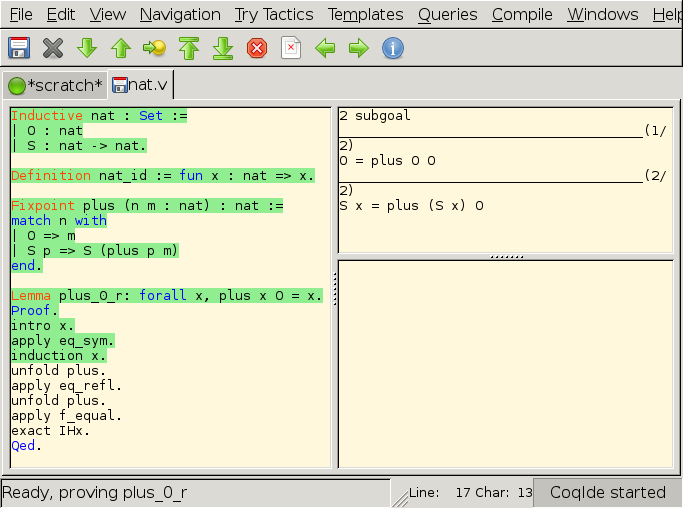
\includegraphics[height=0.78\textheight]{figures/coqide.png}
    \end{center}
    \pnote{
        A computer program can be helpful to prove something formally.\\
        At least you don't need as much paper, and the computer will check every step of the proof.\\
        As probably all of you know, this is a screenshot from the Interactive Theorem Prover Coq.\\
        \\
        It assists the user step-by-step in formulating a proof by checking the validity of each step.\\
        Hence the 'interactive', it requires a user to actually enter the proof steps.
    }
\end{frame}

\begin{frame}{Automated Theorem Proving}
	\begin{center}
        
\includegraphics[width=0.2\textwidth]{figures/alt-ergo.png}\hspace{1em}
        
\includegraphics[width=0.2\textwidth]{figures/eicon.png}\hspace{1em}
        
\includegraphics[width=0.2\textwidth]{figures/prover9t.png}
    \end{center}
    \vspace{5em}
    \bigskip
    First ATP guided proof: Davis, 1957.
    
    \pnote{
        Even better would be when formal proofs can be constructed automatically.\\
        Automated Theorem Provers are capable of doing that.\\
        \\
        In fact, it could be argued that the field of Computing Science was conceived for
        the sake of developing ATP's.\\
        \\
        Several notably ATP's are Alt-Ergo, E, Prover9 and Vampire.\\
        ATP's are however not perfect, and many complex theorems can not be formally proven with just ATP's.\\
        \\
        For Coq there exists some automation in the form of tactics, but these do not ensure full automation.\\
        This is because the logic underpinning Coq is quite expressive and complex, making it difficult to develop an ATP.\\
        \\
        SEG: ATP's are great at proving simple premises, such as proving the correctness of programs.\\
        However, there are also some novel premises being solely proven formally.
    }
\end{frame}

\begin{frame}{Successes of Automated Theorem Proving}
	\begin{block}{Kepler Conjecture}
		What is the best way to stack cannonballs?
		\bigskip
		\begin{center}
				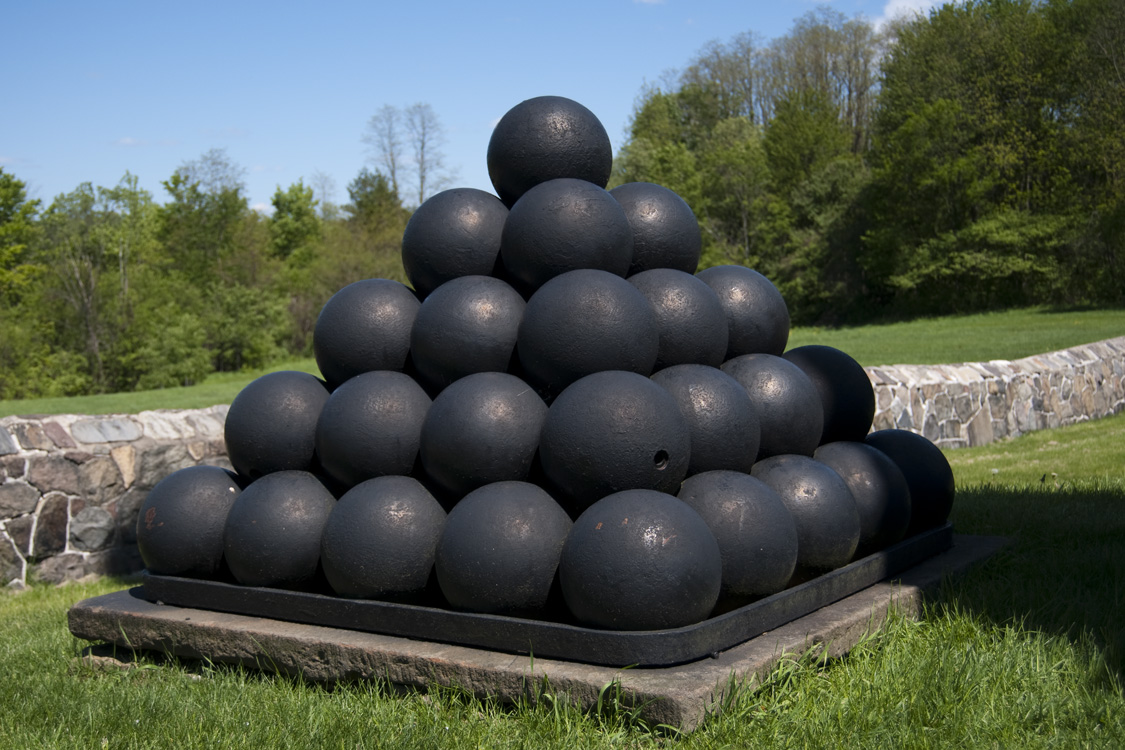
\includegraphics[width=0.5\textwidth]{figures/balls.jpg}\\
				\centering \color{gray}{Nedral (CC by-nc-sa 2.5)}
		\end{center}
		
		\small{
				No arrangement of equally sized spheres has a greater average than $\frac{\pi}{3\sqrt{2}}$.
				Formalized in 2014 by Flyspeck using Isabelle and HOL Light.
        }
        
        \pnote{
            Such as the Kepler Conjecture, \\
            in short a theorem describing the absolute optimal bound to stack cannonballs.
        }
	\end{block}
\end{frame}

\begin{frame}{Hammer Theorem Proving}
	\begin{center}
		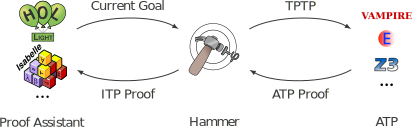
\includegraphics[width=1.0\textheight]{figures/hammer-approach.pdf}
    \end{center}
    \pnote{
        You might ask, why not both?!\\
        That is exactly what the Hammer-approach tries to do.\\
        It translates the theorems and proof goals from an ITP system to that of an ATP system,\\
        and converts the proof back to the ITP system.\\
        \\
        This approach has been applied to various ITP's, such as HOL and Isabelle.\\
		\\
		------------\\
        SEG: and, yes, also Coq!
    }
    \uncover<2->{
        First paper just published!
        \begin{center}
            \bibentry{czajka2018hammer}
        \end{center}
    }
\end{frame}

\begin{frame}{Interactive Theorem Proving}
	\begin{center}
		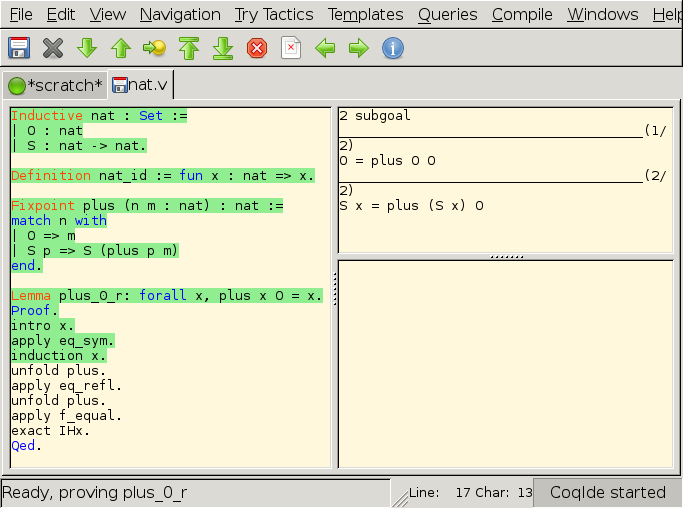
\includegraphics[height=0.78\textheight]{figures/coqide.png}
    \end{center}
    \pnote{
        But this thesis was started a while back, and let's not get ahead of ourselves.\\
        This thesis is about premise selection after all.\\
        \\
        For an ATP, before you can start constructing a proof, you need to know which premises
        are relevant to your proof goal.\\
		Premise selection does just that, it gives advice on what can be used best.\\
		\\
		SEG: and how does this translate to an ITP like Coq?\\
		What other tool makes nice suggestions whilst your editing your document?
    }
\end{frame}

\begin{frame}{Premise Selection in ITP}
	\begin{center}
		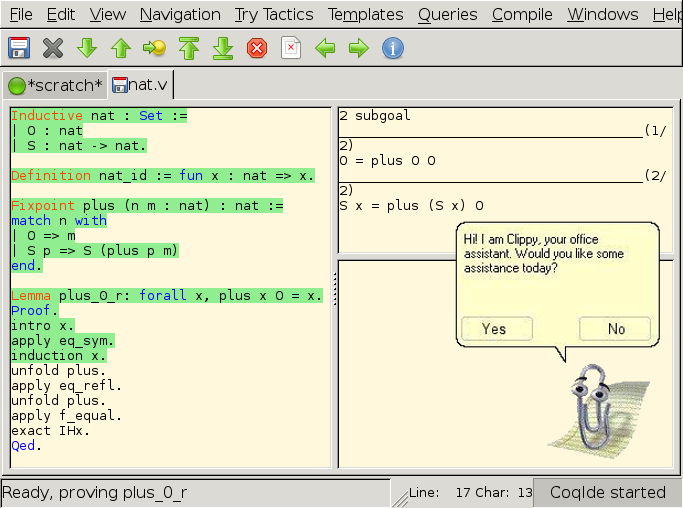
\includegraphics[height=0.78\textheight]{figures/coqide-clippy.png}
    \end{center}
    \pnote{
        Exactly, Clippy.\\
        \\
        But instead on giving advice on how to layout your document,\\
		our premise selection tool sees that you want to prove some property.\\
		\\
		For example, if you're proving a property concerning natural numbers,\\
        it will suggest	 that you use induction on natural numbers.
    }
\end{frame}

\begin{frame}{Source research}
	\begin{center}
		\bibentry{kaliszyk2014machine}
    \end{center}
    \pnote{
        The work in this thesis is based on the work by Cesary Kaliszyk.\\
		Basically I\\
		- read their research,\\
		- implemented their methods,\\
		- reproduced their results,\\
        - and then attempted to implement various likely improvements and other approaches \\
        which could then be compared to the baseline performance of their work.
    }
\end{frame}

\begin{frame}{Roerei}
	Open source and is available from:
	\begin{center}
		\url{https://github.com/Wassasin/roerei}
	\end{center}
	\bigskip
	Design goals of this tool were to:
	\begin{itemize}
		\item Support offline learning and analysis of \machinelearning on the various corpora.
		\item Enable integration in the \coqide GUI.
		\item Enable merging of the premise selection tool in the \coq main branch as a plugin.
    \end{itemize}
    
    \pnote{
        The implementation I made is called Roerei.\\
        Whether the name is a pun I leave as an exercise to the listener.\\
        And the design goal of the implementation is to have a little egg in the corner of your
        Coq IDE giving you suggestions.
    }
\end{frame}

\begin{frame}{How to do Premise Selection for Coq?}
	\begin{center}
		\scalebox{0.4}{
			\begin{tikzpicture}[auto, node distance=2.5cm, main/.style={draw,align=center}]
				\node[main] (coq) {\coqobj[s]\\inside coq};
				\node[main] (xml) [below of=coq] {XML\\representation};
				\node[main] (term) [below of=xml] {\coqobj[s]\\$\name \objdef \term : \type$};
				\node[main] (summary) [below of=term] {Summary\\$<\name[s], \termset{s}, \typeset{s}>$};
				\node[main] (definitions) [below right=2cm and 0cm of summary] {Definitions\\$\defs$};
				\node[main] (theorems) [below left=2cm and 0cm of summary] {Theorems\\$\thms$};
				\node[main] (features) [below of=definitions] {Features\\of theorems\\$\features{}{s}$};
				\node[main] (dependencies) [below of=theorems] {Dependencies\\of theorems\\$\deps{s}$};
				\node[main] (predictor) [below=7.0cm of summary] {Predictor};
		
				\draw[->] (coq) edge node {(1) Coq XML export} (xml);
				\draw[->] (xml) edge node {(2) Parser} (term);
				\draw[->] (term) edge node {(3) Resolver} (summary);
				\draw[->] (summary) edge node [right] {(4) $\bigcup_{s \in S} \typeset{s}$} (definitions);
				\draw[->] (summary) edge node [left] {$\bigcup_{s \in S} \termset{s} \setminus \defs$ (4)} (theorems);
				\draw[dashed] (definitions) edge node {(4)} (theorems);
				\draw[->] (theorems) edge node {(5)} (dependencies);
				\draw[->] (definitions) edge node {(5)} (features);
				\draw[->] (features) edge node [left] {(6)} (predictor);
				\draw[->] (dependencies) edge node [right] {(6)} (predictor);
			\end{tikzpicture}
		}
	\end{center}
    \pnote{
        So how do we do this premise selection?\\
        I'll not be able to explain in full detail everything.\\
        I'll also quickly skip through the slides.\\
        If you feel that it goes too quickly, I have written a thesis.\\
        My apologies beforehand.
    }
\end{frame}


\begin{frame}[fragile]{Gallina}
\begin{lstlisting}[language=Coq, mathescape,basicstyle=\footnotesize,frame=none]
Inductive nat : Set :=
| O : nat
| S : nat -> nat.
Fixpoint plus (n m : nat) : nat :=
match n with
| O => m
| S p => S (plus p m)
end.
Lemma plus_0_r : $\forall$ x , plus x 0 = x.
Proof.
intro x.
apply eq_sym.
induction x.
unfold plus.
apply eq_refl.
unfold plus.
apply f_equal.
exact IHx.
Qed.
\end{lstlisting}
\pnote{
	First, a proof written in Coq is actually written in the language called 'Gallina'.\\
	You may recognize this from the screenshot from earlier.\\
	\\
	It is a small proof concerning natural numbers and that adding 0 to a natural number
	results in the same number.\\
	This example is used throughout this presentation, but also throughout my thesis.
}
\end{frame}

\begin{frame}{\pcic: terms}
	Language on which \coq operates internally.\\
	\bigskip
	\begin{definition}[term]
		A term is a noun or compound word of \pcic.
		A term is typically denoted by $\term$,
		with $\terms$ being the set of all terms.
	\end{definition}
	\bigskip
	\begin{definition}[name]
		A name is an element in the set of names $\names$, and is bound to a term.
	\end{definition}
	\pnote{
		However Coq uses another representation internally called 'pCic', or
		the predicative calculus of (co)inductive constructions.\\
		This is the language on which we are going to base our Premise Selection.\\
		Hence I'll quickly try to show what it looks like.\\
		\\
		In it you have terms (the proofs and transformations).\\
		A term can have a name.
	}
\end{frame}

\begin{frame}{\pcic: types}
	\begin{definition}[type]
		A type is denoted by the semantic subclass of types inside the syntactic class term.
		A type is typically denoted by $\type$, with $\types$ being the set of all types.
	\end{definition}
	\bigskip
	\begin{lemma}
	\coq is based on the Curry-Howard isomorphism.
	Therefor a type is inside the syntactic class term, and all types can also be considered to be terms.
	\[ \types \subseteq \terms \]
	\end{lemma}
	\pnote{
		Each term has a type.\\
		Because Coq is based on the Curry-Howard isomorphism, each type is a term by itself.\\
		Each proof is a term, but the premise it proves is the type of that term.
	}
\end{frame}

\begin{frame}{\pcic: sorts}
	\begin{definition}[sort]
		The type of a type when manipulated as a term is called a sort.
		\pcic uses an infinite well-founded typing hierarchy of sorts,
		with base sorts \sortprop and \sortset,
		and with a family of sorts \sorttype[{i}].
		The set of sorts named $\sorts$ is defined by
		\[\sorts \equiv \{ \sortprop, \sortset, \sorttype[{i}] ~|~ i \in \mathbb{N} \} \]
	
		Their types are defined as
		\[
			\rowcolors{0}{}{}
			\begin{array}{rcl}
				\sortprop & : & \sorttype[1] \\
				\sortset & : & \sorttype[1] \\
				\forall_{i \in \mathbb{N}}~ \sorttype[i] & : & \sorttype[{i+1}]
			\end{array}
		\]
	\end{definition}
	\pnote{
		A type is also typed.\\
		pCic uses an infinite well-founded typing hierarchy of so-called sorts.\\
		Typically a premise is of sort 'prop', a definition of sort 'set', and
		both are again of sort 'type'.\\
		\\
		Question: why well-founded. Due to Russell's Paradox, where a set can not
		be part of itself., hence the number-tagging.\\
		Classically this was a flaw in Cantor's naive set theory.
	}
\end{frame}

\begin{frame}{\gallina: example}
From our natural numbers example the following terms are of sort \sortset:
$$
	\rowcolors{0}{}{}
	\begin{array}{rcl}
		\texttt{0} & : & \texttt{nat} \\
		\texttt{S} & : & \texttt{nat} \rightarrow \texttt{nat}
	\end{array}
$$
$$
	\rowcolors{0}{}{}
	\begin{array}{rclcl}
		\texttt{nat\_id} & \objdef & \lambda x : \texttt{nat}~.~x & : & \texttt{nat} \rightarrow \texttt{nat} \\
		\texttt{plus} & \objdef & \texttt{fix}~\ldots & : & \texttt{nat} \rightarrow \texttt{nat} \rightarrow \texttt{nat} \\
	\end{array}
$$
\pnote{
	So if we quickly look back at our natural-numbers example,\\
	and convert \pcic back to \gallina (such that it still is human readable),\\
	we can see the constructors and their types.\\
	But also the operations.
}
\end{frame}

\begin{frame}{\gallina: example}
From our natural numbers example the following terms are of sort \sortprop:
$$
	\rowcolors{0}{}{}
	\begin{array}{rcl}
		\texttt{nat\_ind} & \objdef & \lambda~P~f_0~f_S ~.~ \texttt{fix}~F~n ~:~ P~n ~:= \\
			&   &  \texttt{match}~ n ~\texttt{with} \\
			&   &  ~~| ~0 => f_0 \\
			&	&  ~~| ~S~m => f_S~m~(F~m) \\
			&	&  \texttt{end} \\
			& : &  \forall P : \texttt{nat} \rightarrow \sortprop,\\
			&   & P~\texttt{0} \rightarrow (\forall n : \texttt{nat},~ P~n \rightarrow P~(\texttt{S}~n)) \rightarrow \forall n : \texttt{nat},~ P~n \\
		\\
		\texttt{plus\_0\_r} & \objdef & \texttt{eq\_sym}
							~~(\texttt{nat\_ind}~(\lambda x~.~\texttt{plus}~x~0)\\
							& & \texttt{eq\_refl}~(\lambda x~\texttt{IH}~.~\texttt{f\_equal}~S~\texttt{IH})~x) \\
							& : & \forall x : \texttt{nat},~ \texttt{plus}~x~0 = x \\
	\end{array}
$$
\pnote{
	The premises look like this.
	The representation of plus_0_r follows from Coq tactics.
}
\end{frame}

\begin{frame}{\pcic: terms}
	\vspace{-0.7em}
	\begin{tabular}{ll}
		$\emptyterm$                                        & Empty term \\
		$\text{Rel}(i:\nat)$                       & Variables as De Bruijn index \\
		$\text{Var}(n:\names)$                     & Named (local) variables \\
		$\text{Evar}(xs:\listtype{\terms}) $        & Existential quantification \\
		$\text{Sort}(n:\names)$                    & Named Sort of types \\
		$\text{Cast}(t:\terms,~ A:\types)$ & Type casting check \\
		$\text{Prods}(x:\names,~ A:\types,~ B:\types$ & $\prod x:A ~.~ B$ \\
		$\text{Lambdas}(x:\names,~ A:\types,~ t:\terms)$   & $\lambda x:A ~.~ t$ \\
		$\text{LetIns}(n:\names,~ t:\terms,~ A:\types)$    & $\text{let~} n := t : A \text{~in~} t$ \\
		$\text{App}(x:\terms,~ ys:\listtype{\terms})$ & Application $x~ys_0 \ldots ys_n$ \\
		$\text{Const}(n:\names,~ S:\sorts)$ & Constant \\
		$\text{Ind}(n:\names,~ S:\sorts)$  & Inductive definition \\
		$\text{Construct}(n:\names,~ S:\sorts)$ & Constructor (of ind. def.) \\
		$\text{Case}(n:\terms,~ t:\terms,~ ys:\listtype{\terms})$ & Deconstruction (of ind. types) \\
		$\text{Fix}(n:\listtype{\names},~ A:\listtype{\types},~ ts:\listtype{\terms})$ & Fixpoint functions \\
		$\text{CoFix}(n:\listtype{\names},~ AS:\listtype{\types},~ ts:\listtype{\terms})$ & Co-fixpoint functions \\
	\end{tabular}
	\pnote{
		But what does pCic actually look like?\\
		A term in pCic is comprised of the following constructors.\\
		\\
		An application, half-way as 'app', is a constructor that takes a term, and several other terms are applied.
	}
\end{frame}

\begin{frame}{\pcic: objects}
	\begin{tabular}{l}
		$\text{Constant}(n:\names,~ t:\terms,~ A:\types)$ \\
		$\text{Variable}(n:\names,~ t:\terms,~ A:\types)$ \\
		$\text{CurrentProof}(n:\names,~ \text{hyps}:\listtype{\listtype{\types} \times \terms}, t:\terms, A:\types)$ \\
		$\text{InductiveConstructor}(n:\names,~ A:\types)$ \\
		$\text{InductiveDefinition}(n:\names,~ A:\types,~ cs:\listtype{\text{InductiveConstructor}})$
	\end{tabular}
	\pnote{
		A term, can be used to define constants, variables, but also proofs in progress.
	}
\end{frame}

\begin{frame}{\xml}
	\lstinline{COQ_XML=-xml COQ_XML_LIBRARY_ROOT=<dest>}
	\lstinputlisting[language=xml,basicstyle=\tiny]{figures/plus.con.xml}
	\pnote{
		And old versions of Coq (currently no longer) supported exporting these\\
		pCic versions to XML, which looks like this.\\
		As a very first step, my tool exports Gallina scripts to this XML using the Coq compiler as seen above.
	}
\end{frame}

\begin{frame}{Parsing}
	\lstinputlisting[language=caml,basicstyle=\tiny]{figures/plus.con.types.txt}
	\pnote{
		Then this XML is converted to something like this.
	}
\end{frame}

\begin{frame}{Extraction}
	\vspace{-2.55em}
	\[c : \terms \rightarrow \nat \rightarrow \listtype{\names \times \nat} \]
	\bigskip
	\hspace{-1.7em}
	\begin{tabularx}{\textwidth}{ll}
		$c(\emptyterm, d)$              & $ = \nil $ \\
		$c(\text{ARel}(\cdots), d)$     & $ = \nil $ \\
		$c(\text{AVar}(u), d)$          & $ = \singleton{(u, d)} $ \\
		$c(\text{AEvar}(l), d)$         & $ = \flattenlist{\map{l}{\lambda x . c(x, d+1)}} $ \\
		$c(\text{ASort}(\cdots), d)$    & $ = \nil $ \\
		$c(\text{ACast}(t, A), d)$      & $ = \concat{c(t, d+1)}{c(A, d+1)} $ \\
		$c(\text{AProds}(l, t), d)$     & $ = c_{\times}(l, t, d) $ \\
		$c(\text{ALambdas}(l, t), d)$   & $ = c_{\times}(l, t, d) $ \\
		$c(\text{ALetIns}(l, t), d)$    & $ = c_{\times}(l, t, d) $ \\
		$c(\text{AApp}(l), d)$  & $ = \left(
		  \begin{array}{l}
			\singleton{(\text{special:app}, d)} ~\concatsymbol \\
			\map{l}{ \lambda a . c(a, d+1) }
		  \end{array}
		  \right)
		  $ \\
		$c(\text{AConst}(\cdots, u), d)$  & $ = \singleton{(u, d)} $ \\
		$c(\text{AInd}(\cdots, u), d)$  & $ = \singleton{(u, d)} $ \\
		$c(\text{AConstruct}(\cdots, u), d)$  & $ = \singleton{(u, d)} $ \\
		$c(\text{ACase}(u, A, i, l), d)$  &
		  $= \left(
			\begin{array}{l}
			  \concat{\singleton{(u, d)}}{
				\concat{c(A, d+1)}{c(i, d+1)}
			  }
			  ~\concatsymbol \\
			  \flattenlist{ \map{l}{\lambda x . c(x, d+1)} } \\
			\end{array}
			\right)
		  $ \\
		$c(\text{AFix}(l), d)$        & $ = c_{\text{fix}}(l, d) $ \\
		$c(\text{ACoFix}(l), d)$      & $ = c_{\text{fix}}(l, d) $ \\
	\end{tabularx}
	\pnote{
		And then I throw everything away.\\
		\\
		\\
		Well, all the structure at least.\\
		The names used in each term are kept and counted.
	}
\end{frame}

\begin{frame}{Extraction}
	$$
		\rowcolors{0}{}{}
		\begin{array}{lcl}
		c_{\times}(l, t, d) & = &
			c(t, d+1) ~\concatsymbol \\
			& & \map{l}{ \lambda (n, a) ~.~ \cons{(\text{special:prod}, d)}{c(a, d+1)}} \\
		c_{\text{fix}}(l, d) & = & \flattenlist{ \map{l}{ \lambda (A, t) ~.~ \concat{c(A, d+1)}{c(t, d+1)} } }
		\end{array}
	$$
	\pnote{
		I'll not go into detail.
	}
\end{frame}

\begin{frame}{Extraction}
	\hspace{-1em}\vbox{\begin{tabular}{ll}
		$c_{\text{type}}(\text{AConstant}(n, A, t))$ & $= c(A, 0)$ \\
		$c_{\text{type}}(\text{AIndDef}(n, l))$ & $= \flattenlist{
			\map{l}{
				\hspace{-0.5em}\begin{array}{l}
					\lambda (A, m) ~.~ c(A, 0) ~\concatsymbol\\
					\flattenlist{\text{map}(m, \lambda x . c(x, 0))}
				\end{array}
			}
		} $\\
		$c_{\text{type}}(-)$ & $= \nil $ \\
		$c_{\text{term}}(\text{AConstant}(n, A, t))$ & $= c(t, 0)$ \\
		$c_{\text{term}}(-)$ & $= \nil $ \\
	\end{tabular}}
	\pnote{
		And then you can count everything for just terms and just the types.
	}
\end{frame}

\begin{frame}{Extraction}
	\begin{definition}[Flatten symbols $\flattensym$]
	$
		\rowcolors{0}{}{}
		\arraycolsep=0.2em
		\begin{array}{lcl}
		\flattensym & : & \terms \rightarrow 2^{\names} \\
		\flatten{t} & = & \foldr{\lambda (n, d)~s ~.~ \{n\} \cup s}{\varnothing}{c(t, 0)}
		\end{array}
	$
	\end{definition}
	\pnote{
		You can record just the occurance of terms and types.
	}
\end{frame}

\begin{frame}{Extraction}
	\begin{definition}[Count symbols $\countoccursym$]
	$
	\rowcolors{0}{}{}
	\arraycolsep=0.2em
	\begin{array}{lcl}
		\countoccursym & : & \terms \rightarrow \nat^{\names} \\
		\countoccur{t} & = & \lambda n ~.~ \foldr{\lambda (m, d)~s ~.~ \text{if~} n = m \text{~then~} s+1 \text{~else~} s}{0}{c(t, 0)}
	\end{array}
	$\\
	\end{definition}
	\bigskip
	\begin{definition}[Depth of symbols $\depthoccursym$]
	$
		\rowcolors{0}{}{}
		\arraycolsep=0.2em
		\begin{array}{lcl}
		\depthoccursym & : & \terms \rightarrow \names \rightharpoonup \nat \\
		\depthoccur{t} & = & \lambda n ~.~ \foldr{\lambda (m, d)~s ~.~ \text{if~} n = m \text{~then~} f(d, s) \text{~else~} s}{\infimum}{c(t, 0)} \\
		\end{array}
	$\\
	\bigskip
	$
		\rowcolors{0}{}{}
		\text{with~} \begin{array}{l}
			f(d, \infimum) = d \\
			f(d, s) = \text{min}(d, s) \\
		\end{array}
	$
	\end{definition}
	\pnote{
		But you can also count the number of occurances, or record the depth of their occurance.
	}
\end{frame}

\begin{frame}{What do we currently have?}
	A summary with for each named term
	\begin{itemize}
		\item which other named terms have been used to define it.
		\item the frequency of the occurance.
		\item the depth of the occurance.
	\end{itemize}
\end{frame}

\begin{frame}{What do we want?}
	Given a proof goal, which premises will help me prove the goal.
	\pnote{
		So we're not quite there yet.\\
		\\
		We've only made all the information Coq has more accessible.
	}
\end{frame}

\begin{frame}{Theorems and definitions}
	\begin{definition}[Theorem]
		A type that has been proven, along with the term that proves it.
	\end{definition}
	\bigskip
	\begin{definition}[Definition]
		A term (which has a type) that is not a theorem.
		Thus it can only be transformative or a simple constant.
	\end{definition}
	\pnote{
		Let's make a distinction.\\
		\\
		We have named terms which form a proof: theorems.\\
		But we also have terms which are just mechanisms which help us:\\
		we'll call those definitions.
	}
\end{frame}

\begin{frame}[fragile]{Theorems and definitions}
	\coq has a sort for theorems: \sortprop.
	\pause
	\bigskip
\begin{lstlisting}[language=Coq, mathescape]
Notation "'CProp'" := Type.
\end{lstlisting}
	\bigskip
	Thus for \corn the sort of a theorem is \sorttype{}$(n+1)$.
	\pnote{
		I have a great idea!\\
		Let's use that sort, Prop!\\
		--------\\
		However some Coq libraries, such as CoRN (Coq Constructive Repository at Nijmegen), which originated right here,
		do not use the sort Prop at all.\\
		Thus that will not work.
	}
\end{frame}

\begin{frame}{Heuristic}
	Premise: a theorem concerning theorems in \coq is not useful.
	\bigskip
	\begin{definition}[$\defs$]
		All names occuring in types cannot be theorems, and thus must be definitions.
		\[ \defs = \bigcup_{s \in \objs} \typeset{s} \]
	\end{definition}
	\bigskip
	\begin{definition}[$\thms$]
		Theorems build upon eachother, thus what is used in terms, except the definitions, must be theorems.
		\[ \thms = (\bigcup_{s \in \objs} \termset{s}) \setminus \defs \]
	\end{definition}
	\pnote{
		Kaliszyk uses a heuristic to solve this issue.\\
		Theorems prove stuff concerning definitions, mechanisms, not concerning other theorems.\\
		And because the type of a proof is the proposition of the proof, only definitions may occur in those types.\\
		\\
		Theorems build upon eachother, thus theorems will occur in the terms of proofs.\\
		And anything that is a definition can never be a theorem.\\
		\\
		This heuristic works really well.
	}
\end{frame}

\begin{frame}{What do we currently have?}
	\begin{itemize}
		\item Definitions: the subjects of proofs.
		\item Theorems: the objects of proofs and proofs themselves.
	\end{itemize}
\end{frame}

\begin{frame}{What do we want?}
	Given a proof goal, which premises will help me prove the goal, and how likely?
	\pnote{
		How are we going to do Premise Selection?\\
		I've changed it a bit.\\
		This sounds like something involving statistics...
	}
\end{frame}

\begin{frame}{Features and dependencies}
	\begin{definition}[Features]
		For object $s$ yield whether definition $x \in \defs$ is used in the type of $s$.
		\[ \features{}{s}(x) = \flatten{\type[s]}(x) \]
	\end{definition}
	\bigskip
	\begin{definition}[Dependencies]
		For object $s$ yield whether theorem $x \in \thms$ is used in the term of $s$.
		\[ \deps{s}(x) = \flatten{\term[s]}(x) \]
	\end{definition}

	\pnote{
		We are going to do machine learning, thus we need to define our dataset.\\
		...\\
		Yes, you are in a machine learning talk.\\
		Actually, there is a separate field of ATP's using machine learning.\\
		The Hammers are an example of that.\\
		\\
		Anyway,\\
		Our features are our definitions, as they describe how premises look (i.e. what they prove)\\
		\\
		Now, our classes in our ranking, to use machine learning terms, are the premises that
		can be used to prove the goal. \\
		These premises are called dependencies, as their theorems are dependant on these premises
		to form their proofs.
	}
\end{frame}

\begin{frame}{Predictors}
	Given a proof goal $\in \types$, 

	\begin{definition}[Ranking $r \in \rankings$]
		We want to yield a ranking of dependencies.
		\[ r : \depset \rightharpoonup \mathbb{R} \]
	\end{definition}
	\bigskip
	\begin{definition}[Predictor $p \in \predictors$]
		And we generate rankings using a predictor.
		\[ p : \types \rightarrow \rankings \]
	\end{definition}
\end{frame}

\begin{frame}{Example: \knn}
	\begin{definition}[Euclidean distance]
		$ \text{dist}(x, y) = \left( \sum_{i \in \featurekeys} \left( \features{}{x}(i) - \features{}{y}(i) \right)^2 \right)^{\frac{1}{2}} $
	\end{definition}
	\bigskip
	\begin{definition}[Predicate $x$ is closer to $\phi$ than $y$]
	$ \text{closer}_\phi(x, y) = \text{dist}(x, \phi) \leq \text{dist}(y, \phi) $
	\end{definition}
	\bigskip
	\begin{definition}[Yield the $n^{\text{th}}$ element]
	$
	\rowcolors{0}{}{}
    \nth{n}{X} = \left\{
      \begin{array}{ll}
        \infimum_X & \text{if}~n = 0 \\
        \nth{n-1}{X \cap \infimum_X} & \text{if}~n > 0 \\
      \end{array}
    \right.
	$
	\end{definition}
	\bigskip
	\begin{definition}[Yield the closest $K$ elements to $c$]
	$
    \text{closest}_K(c) = \downset{S}{\nth{K}{(S, \text{closer}_c)}}
	$
	\end{definition}
	\pause
	\bigskip
	\begin{definition}[\knn]
	$
    	P^K_\text{knn}(c, \phi) = \sum_{x \in \text{closest}_K(c)} \deps{x}(\phi) \times \text{dist}(c, x)
	$
	\end{definition}
	\pnote{
		A simple example of a predictor uses something akin to KNN.\\
		In the thesis I've defined everything in the following manner.\\
		\\
		Naturally the C-code looks quite different.\\
		-----\\
		At the bottom you'll see how it is defined in the end.\\
		\\
		I've defined several of these predictors in the thesis.\\
		Now we're done!\\
		We have premise selection!
	}
\end{frame}

\begin{frame}{Estimating performance}
	Used: 10-fold \crossvalidation (same as source)\\
	\bigskip
	\pause
	\textbf{Problem}: A predictor might use a theorem that can not yet be proven.\\
	\bigskip
	Implemented 3 different schemes: canonical, pessimistic and optimistic.
	\pnote{
		So given a known library, such as the Coq standard library,\\
		you can now try to estimate how well your implementation performs.\\
		\\
		In Machine Learning you have a cross validation to rule out bias, and to better approximate
		the performance on an previously unseen dataset.\\
		\\
		-----\\
		However, this is not a simple dataset.\\
		Using a not yet seen theorem to generate premise selection suggestions can be considered cheating.\\
		To solve this...
	}
\end{frame}

\begin{frame}{Estimating performance: canonical method}
	Construct a poset from $\objs$ using the dependency relation for $x, y \in \objs$:
	\[ x <_D y ~~\leftrightarrow~~ \depstrans[x] \cap (\parentstrans[y] \cup \{y\}) \neq \emptyset \]\\
	Linearize with Depth-first topological sort using $<_D$ to provide extra context.\\
	\bigskip
	Given a conjecture $\phi \in \testset$,
	\[ \trainset^{\phi} = \{ x \in \trainset | x < \phi \} \]
	\pnote{
		The canonical method best approximates using a directed acyclic graph as
		often seen in import strategies of most programming languages and indeed Gallina.\\
		\\
		However this method also supports randomizing this import order, and still be able to
		create separate train and testsets.
	}
\end{frame}

\begin{frame}{Metrics}
	Given $r \in \rankings$,\\
	\bigskip
	\begin{definition}[Suggestions]
	$ \suggestions{r} = \{ d \in \depset ~|~ r(d) ~\text{is defined} \} $
	\end{definition}
	\bigskip
	\begin{definition}[Best suggestions]
	$ \topn{n}{r} = \downset{\depset}{\nth{n}{(\suggestions{r}, \lambda x~y. r(x) > r(y))}} $
	\end{definition}
	\bigskip
	\begin{definition}[\oocover]
	$\oocoverf{r}{s} = \frac{ |\topn{100}{r} \bigcap \deps{s}| } { |\deps{s}| } $
	\end{definition}
	\pnote{
		Next up is actually gaining performance metrics.\\
		I've been notified that in other fields these metrics have different names, namely 100cover and recall@100.\\
		\\
		The two most commonly used metrics are recall@100 and auc.\\
		Basically recall@100 is the ratio of how many of the first 100 suggestions/guesses are correct.
	}
\end{frame}

\begin{frame}{Metrics}
	\begin{definition}[Index]
		$
		\rowcolors{0}{}{}
		\findindex{X}{x} = \left\{
		\begin{array}{ll}
			0 & \text{if~} x = \infimum_X \\
			\findindex{X \cap \infimum_X}{x}+1 & \text{if~} x \neq \infimum_X \\
		\end{array}
		\right.
		$
	\end{definition}
	\bigskip
	\begin{definition}[Area Under Curve (AUC)]
	$
	\aucf{r}{s} = \frac{
		\sum_x^X \sum_y^Y {\findindex{\suggestions{s}}{x} < \findindex{\suggestions{s}}{y}}
	}{
		|X| \times |Y|
	}
	$ \\
	\bigskip
	$
	\rowcolors{0}{}{}
	\begin{array}{ll}
		\text{where~} & X = \suggestions{r} \bigcap \required[s] \\
		& Y = \suggestions{r} - \required[s] \\
	\end{array}
	$
	\end{definition}
	\pnote{Integral}
\end{frame}

\begin{frame}{Contributions}
	\begin{itemize}
		\item Precise definition of approach.
		\item Fast implementation in C++.
		\item Application to multiple corpora (libraries).
		\item Experiments with various features.
		\item Novel adaptation of method Adarank / Learning to Rank.
		\item Varying estimations of performance.
		\item Investigated the importance of prior knowledge.
	\end{itemize}
	\pnote{
		What I've described up until now has also been done by Kaliszyk.\\
		Here I highlight in what way my thesis distinguises itself from this prior work.\\
		\\
		Corpora: Coqstdlib, Formalin (by Robbert Krebbers), CoRN, Mathclasses and Mathcomp.\\
		\\
		Question: why own C++ implementation?\\
		Given differing performance estimators is not feasible to do with python/scikit.\\
		Cache locality a big factor.\\
		Cardinality important factor. (matrix 50000 * 10000, 500mil)
	}
\end{frame}

\begin{frame}{Corpora}
	\begin{center}
		\begin{tikzpicture}[auto, node distance=2.5cm, main/.style={align=center}]
			\node[main] (coq) {\coq};
			\node[main] (mathclasses) [right=2cm of coq] {\mathclasses};
			\node[main] (formalin) [above=0.5cm of mathclasses] {\formalin};
				\node[main] (mathcomp) [below=0.5cm of mathclasses] {\mathcomp};
			\node[main] (corn) [right=1.5cm of mathclasses] {\corn};

			\draw[->] (coq) to [out=0,in=180] (formalin);
			\draw[->] (coq) to [out=0,in=180] (mathcomp);
			
			\draw[->] (coq) to [out=0,in=180] (mathclasses);
			\draw[->] (mathclasses) to [out=0,in=180] (corn);
		\end{tikzpicture}
	\end{center}
	\pnote{
		Coq libraries are dependant on eachother.\\
		I've investigated whether it helps to include or exclude parts of dependant corpora.\\
		Surprisingly, it is better to leave out as much of prior data as possible.
	}
\end{frame}

\begin{frame}{Results (\knn)}
	\vbox{
	\begin{tikzpicture}
		\begin{axis}[
			xlabel=$k$,
			ylabel=\oocover,
			legend pos=outer north east,
			thick,
			cycle list name=Set1-5,
			width=\textwidth,
			height=5cm,
			width=10cm,
			legend style={at={(0,-0.45)},anchor=north west},
		  ]
	
		  \addplot+[smooth, no markers] table [y index=1] {data/knn-coq-frequency-canonical.dat};
		  \addlegendentry{\coq}
	
		  \addplot+[smooth, no markers] table [y index=1] {data/knn-ch2o-frequency-canonical.dat};
		  \addlegendentry{\formalin}
	
		  \addplot+[smooth, no markers] table [y index=1] {data/knn-mathclasses-frequency-canonical.dat};
		  \addlegendentry{\mathclasses}
	
		  \addplot+[smooth, no markers] table [y index=1] {data/knn-corn-frequency-canonical.dat};
		  \addlegendentry{\corn}
	
		  \addplot+[smooth, no markers] table [y index=1] {data/knn-mathcomp-frequency-canonical.dat};
		  \addlegendentry{\mathcomp}
		\end{axis}
	\end{tikzpicture}
	}
	\pnote{
		To show you some differences in how Roerei behaves for each corpus,
		here is the performance for KNN for each corpus.\\
		Not that Formalin performance is highest, and CoRN performance is lowest.\\
		\\
		This is probably due to the fact that Formalin has less complex proofs, mostly
		deconstructing inductive definitions.\\
		Whereas CoRN is a collection of formalized mathmatical proofs,
		which ought to be less straight-forward.
	}
\end{frame}

\begin{frame}{Results (Corpora)}
	\vspace{-0.3cm}
	\hspace{-1.1cm}
	\vbox{
	\begin{tikzpicture}
		\begin{axis}[
			width=13cm,
			height=5cm,
			ymajorgrids,
			ybar,
			every axis plot/.append style={fill},
			ylabel={\oocover},
			symbolic x coords={{coq},{corn},{formalin},{mathclasses},{mathcomp}},
			xtick=data,
			xticklabels={{\coq},{\corn},{\formalin},{\mathclasses},{\mathcomp}},
			x tick label style={rotate=45,anchor=east},
			legend style={at={(0,-0.45)},anchor=north west},
			cycle list name=Set1-5
		]
		\addplot table[header=false] {data/best-knn-canonical.dat};
		\addlegendentry{\knn}
		\addplot table[header=false] {data/best-knn_adaptive-canonical.dat};
		\addlegendentry{\knnadaptive}
		\addplot table[header=false] {data/best-naive_bayes-canonical.dat};
		\addlegendentry{\nb}
		\addplot table[header=false] {data/best-ensemble-canonical.dat};
		\addlegendentry{\ensemble}
		\addplot table[header=false] {data/best-adarank-canonical.dat};
		\addlegendentry{\adarank}
		\end{axis}
	\end{tikzpicture}
	}
	\pnote{
		This is the same graph, but instead of just for KNN it is for all predictors I've implemented.\\
		Note that Adarank performs best in all cases.\\
		Unfortunately it is also computationally a lot more expensive.\\
		\\
		The same behaviour can be seen across all predictors with regards to performance
		for each corpus.
	}
\end{frame}

\begin{frame}{Results (prior knowledge)}
	\begin{figure}[H]
		\centering
		\footnotesize
		\begin{tabular}{r|cll}
		Method & mode & \oocover & \auc \\\hline
		\knn K=40 & prior & 0.421 & 0.538\\
\knn K=56 & without & 0.440 ({\color{green}+4.4\%}) & 0.569 ({\color{green}+5.5\%})\\
\knn (adaptive) & prior & 0.312 & 0.627\\
\knn (adaptive) & without & 0.372 ({\color{green}+16.1\%}) & 0.670 ({\color{green}+6.5\%})\\
\nb $\pi=80$ $\sigma=-18$ $\tau=0$ & prior & 0.539 & 0.722\\
\nb $\pi=80$ $\sigma=-15$ $\tau=0$ & without & 0.544 ({\color{green}+0.9\%}) & 0.721 ({\color{red}-0.2\%})\\
\adarank T=7 & prior & 0.583 & 0.832\\
\adarank T=5 & without & 0.576 ({\color{red}-1.2\%}) & 0.796 ({\color{red}-4.5\%})\\
\ensemble & prior & 0.538 & 0.750\\
\ensemble & without & 0.543 ({\color{green}+1.0\%}) & 0.761 ({\color{green}+1.4\%})\\

		\end{tabular}
		\caption{Results for the \corn (frequency) dataset with canonical strategy, with prior knowledge compared to without}
	\end{figure}
	\pnote{
		Also interesting is the effect on including knowledge from prior corpora.\\
		So for example including results from the Coq stdlib when testing the performance
		of Formalin, or in this case, CoRN.\\
		Surprisingly, not including this prior knowledge improves the performance.\\
		So maybe a filter that detects irrelevant data can help the performance a lot.
	}
\end{frame}

\begin{frame}{Results (relative to Kaliszyk)}
	\small
	\tabcolsep=0.2em
	\begin{tabular}{lcccccc}
		 & \oocover & (ours) & & \auc & (ours) & \\
		\hline
		\knnadaptive & 0.723 & 0.390 & ({\color{red}-46.1\%}) & 0.834 & 0.695 & ({\color{red}-16.6\%})\\
\nb & 0.726 & 0.583 & ({\color{red}-19.7\%}) & 0.836 & 0.803 & ({\color{red}-4.0\%})\\
\ensemble & 0.749 & 0.586 & ({\color{red}-21.8\%}) & 0.849 & 0.811 & ({\color{red}-4.5\%})\\
\adarank & - & 0.641 & ({\color{red}-14.4\%}) & - & 0.894 & ({\color{green}+5.3\%})\\

	\end{tabular}
	\pnote{
		Finally, how did we do?\\
		As you can see, across the board we have worse performance compared to Kaliszyk.\\
		\\
		This is odd, as I've set out to reproduce their work in the first place.\\
		\\
		I am not able to give a proper explanation as to why this is.\\
		Unfortunately the source code of their tooling is no longer available, so I am not able
		to investigate this further in a constructive manner.
	}
\end{frame}

\begin{frame}{Reproducibility}
	\begin{center}
        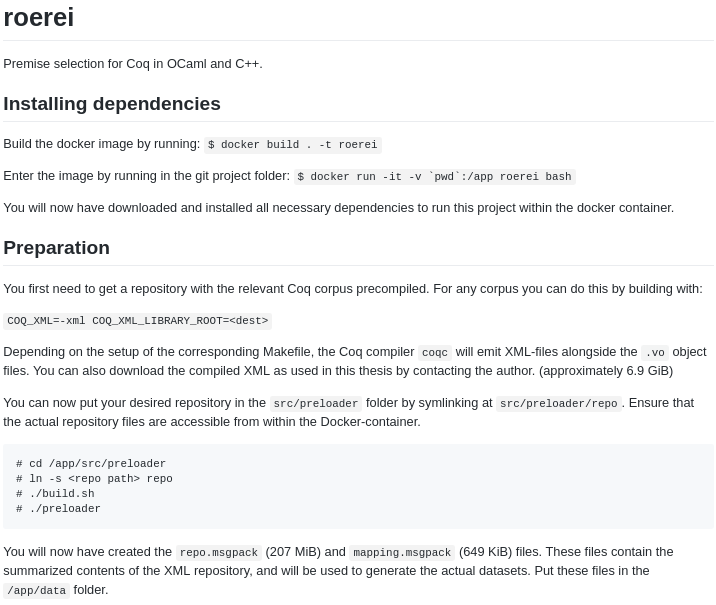
\includegraphics[width=0.7\textwidth]{figures/github.png}
    \end{center}

	\pnote{
		Luckily nowadays it is required at the RU to publish your dataset and code in a repository.\\
		I've written documentation and provide docker images to enable the continuation of my research.
	}
\end{frame}

\begin{frame}{Thank you!}
	\begin{center}
        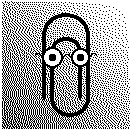
\includegraphics[width=0.6\textwidth]{figures/vigor.png}
    \end{center}

	\pnote{
		Luckily nowadays it is required at the RU to publish your dataset and code in a repository.\\
		I've written documentation and provide docker images to enable others to continue with my research.
	}
\end{frame}

\end{document}
